\documentclass[17pt,margin=0.5in,innermargin=-2.5in,blockverticalspace=1cm]{tikzposter}
\geometry{paperwidth=40in,paperheight=31in}
\usepackage[utf8]{inputenc}
\usepackage{amsmath}
\usepackage{amsfonts}
\usepackage{amsthm}
\usepackage{amssymb}
\usepackage{mathrsfs}
\usepackage{graphicx}
\usepackage{adjustbox}
\usepackage{enumitem}
\usepackage[backend=biber,style=numeric]{biblatex}
%\usepackage[square,sort,comma,numbers]{natbib}

\usepackage{tikz-feynman}

\usepackage{wrapfig}

\AtBeginBibliography{\small}
\addbibresource{Bibliography.bib}

% set theme parameters
\tikzposterlatexaffectionproofoff
\usetheme{Default}
\usecolorstyle{Default}

\title{\Huge On Various Parametrizations of Feynman Integrals}
\author{\Huge Giovanni Ossola, Ray D. Sameshima}
\institute{\Huge \emph{Physics Department}}

\begin{document}
\maketitle

\node [below right=1cm and 2cm] at (bottomleft |- topright) {
\includegraphics[width=6cm]{citytechlogo_blue.jpg} \, 
\includegraphics[width=6cm]{CTP.png} };
\node [below left=1cm and 5cm] at (topright) {
\includegraphics[width=5cm]{NSF_4-Color_bitmap_Logo.png}\, 
\includegraphics[width=5cm]{GC.png} };

\centering
\begin{columns}
    \column{0.33}
    \block{Abstract}{
        \textcolor{red}{Scattering amplitudes} in quantum field theories allow us to compare the phenomenological prediction of theoretical models with the measurement data at collider experiments. 
        Feynman diagrams and the related Feynman rules allow us to write scattering amplitudes in terms of a class of Integrals over momentum space, known as \textcolor{red}{Feynman Integrals}. 
        In our poster, we discuss two different parametrizations of Feynman Integrals, namely \textcolor{red}{Lee-Pomeransky} and \textcolor{red}{Baikov} parametrization. 
        By going to different parametrizations, we do not simply choose different variables to represent the same multidimensional integral, the gain is much higher: some properties of Feynman integrals, and more in general, scattering amplitudes, become particularly transparent when we use the appropriate parametrization. 
        Indeed, the \textcolor{red}{Lee-Pomeransky} parametrizations clarifies some graph-theoretical properties which Feynman graphs intrinsically have, and Baikov parametrization gives us geometrical interpretations of Feynman integrals through Gram-determinants. 
        We also show that, in these parametrizations, the famous \textcolor{red}{Cauchy's integral formula} can provide a recipe to handle negative exponents in the denominators of Feynman integrals; the price we have to pay for this procedure is simply a dimensional shift.
    }
    
    \block{Feynman Integrals}{
        A \textcolor{red}{scattering amplitude} is given in a diagram form $\to$ \textcolor{red}{Feynman diagrams}:
        \begin{equation}
        \nonumber
        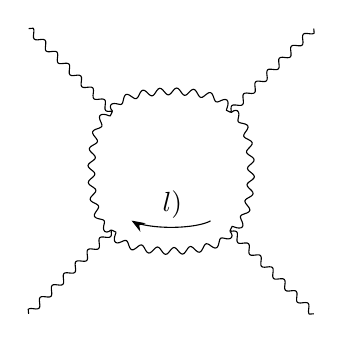
\begin{tikzpicture}[baseline=(current bounding box.center)]
        \begin{feynman}
          \vertex (k2) ;
          \vertex [below right=of k2] (c);
          \vertex [right=of c] (d);
          \vertex [above right=of d] (k3);
          \vertex [below=of c] (b);
          \vertex [right=of b] (a);
          \vertex [below left = of b] (k1);
          \vertex [below right = of a] (k4);
          
          \diagram* {
            (a) -- [boson] (k4),
            (b) -- [boson] (k1),
            (c) -- [boson] (k2),
            (d) -- [boson] (k3),
            (a) -- [boson, half left, looseness=0.6, momentum'=\(l\))] (b),
            (b) -- [boson, half left, looseness=0.6] (c),
            (c) -- [boson, half left, looseness=0.6] (d),
            (d) -- [boson, half left, looseness=0.6] (a),
          };
        \end{feynman}
        \end{tikzpicture}
        \mapsto
        \int d^dl \frac{N(l)}{D_1 D_2 D_3 D_4}
        \end{equation}
        This translation can be achieved by means of Feynman rules.
        
        It is well-known that we can decompose a Feynman Integral into a linear combination of scalar integrals.~\cite{Passarino:1978jh, Tarasov:1996br, Tarasov:1997kx,Mastrolia:2011pr, Grozin:2011mt}
        We, therefore, consider a family of $L$-loops scalar integrals:
        \begin{equation}
            \nonumber
            I(\vec{\nu}) := \left( \prod_{a=1}^{L} \int \frac{d^d l_a}{(2\pi)^d} \right) \frac{1}{D_1^{\nu_1} \cdots D_N^{\nu_N}} \, .
        \end{equation}
    }
    
    \block{Baikov Parametrization}{
        
        Under the integration variable change
        \begin{align*}
        (l_1, \cdots, l_L) \mapsto (D_1, \cdots, D_N),
        \end{align*}
        we obtain~\cite{Baikov:1996iu, Grozin:2011mt} the following parametrization:
        \begin{align*}
        I(\vec{\nu}) \sim \int \frac{d D_1 \cdots dD_N}{D_1^{\nu_1} \cdots D_N^{\nu_N}} P^{\frac{d-L-E-1}{2}}
        \end{align*}
        where $P$ is the Jacobi determinant of this variable change
        \begin{align}
        \nonumber
        P &= \det \left[ q_i \cdot q_j \right] (D_1,\cdots, D_N)
        \end{align}
        that is, the determinant of scalar products expressed as a polynomial of denominators, and this $P$ is called  the \textcolor{red}{Baikov polynomial}.
        The integration domain is determined by the zeros of $P$.
        
        $P$ and the integration domain do not depend on the indices $\nu_1, \cdots, \nu_N$, so the family of integrals are characterized by a polynomial $P$.

    }
    
    \block{Acknowledgements}{
    
        This project has been supported by the National Science Foundation under
        Grant PHY-1417354.
        We would like to thank Hjalte Frellesvig, Federico Gasparotto, Manoj K. Mandal, Pierpaolo Mastrolia, Luca Mattiazzi, for fruitful discussions.
        %RDS 
        We would also like to thank the organizers of "The Mathematics of Linear Relations between Feynman Integrals." 
        
    }
    
%%%%%%%%%%%%%%%%%%%%%%%%%%%%%%%%%%%%%%%%%%%%%%%%%%%%%%%%%%%

    \column{0.33}
    \block{Lee-Pomeransky Parametrization}{
    
        We can show the scalar integrals becomes
        \begin{align*}
        I(\vec{\nu}) \sim 
        \prod_{a=1}^N \int_0^\infty  \frac{dx_a x^{\nu_a-1}}{\Gamma(\nu_a)} \mathcal{G}^{-d/2}
        \end{align*}
        of \textcolor{red}{Lee-Pomeransky parametrization}~\cite{Lee:2013hzt}, where Lee-Pomeransky polynomial
        \begin{align*}
        \mathcal{G} := \mathcal{U} + \mathcal{F} 
        \end{align*}
        and two \textcolor{red}{graph polynomials} are defined as
        \begin{align*}
        \mathcal{U} := \det A, \,
        \mathcal{F} := \det \begin{pmatrix} A & B \\ B^t & C \end{pmatrix}
        \end{align*}
        and the associated matrices are given in the following quadratic form:
        \begin{align*}
        \sum_a^N x_a D_a = l^t A l +  2B^t l + C.
        \end{align*}
        This polynomial $\mathcal{G}$ does not depend on indices and characterizes the family of integrals.

        We can also show that these polynomials can be derived through graph-theoretically,~\cite{nakanishi1971graph} i.e., they depend only on the Feynman graph.
        These polynomials, indeed, reflect the graph-theoretical symmetry of Feynman graph; for example, if the graph has swap symmetry of internal lines, the polynomials are symmetric under the corresponding parameters.
    
    }
    
    \block{IBP-like identities over LP}{
    Through the following functional:
        \begin{equation}
        \nonumber
            G_i(f)=
            \int dx_1 \ldots \int dx_N\ \partial_i \left[ f \mathcal{G}^{-\frac{d}{2} +1} \right]
            = S_i(f)\, ,
        \end{equation}
    we can build a set of linear equations.
    On the one hand, we apply the \textcolor{red}{partial derivative} to obtain a linear combination of integrals with full $N$ denominators:
    \begin{equation}
        \nonumber
        G_i(f) =
        \int dx_1 \ldots \int dx_N\ \underbrace{\partial_i \left[ f \mathcal{G}^{-\frac{d}{2} +1} \right]}_{\text{partial derivative}}\, ,
    \end{equation}
    On the other hand, we use the \textcolor{red}{fundamental theorem of calculus} to associate this functional with the surface term; under dimensional regularization scheme, we can identify this surface term as another linear combination of integrals that has no $D_i$:
    \begin{equation}
        \nonumber
        S_i(f)=
            \left(\prod_{a\neq i}\int dx_a \right) \underbrace{ \int dx_i \partial_i}_{\text{surface term}} \left[ f \mathcal{G}^{-\frac{d}{2} +1} \right]\, .
    \end{equation}
    
    }
    
    \block{References}{
        \vspace{1em}
        \begin{center}\mbox{}\vspace{-\baselineskip}
            \printbibliography[heading=none]
        \end{center}
    }

%%%%%%%%%%%%%%%%%%%%%%%%%%%%%%%%%%%%%%%%%%%%%%%%%%%%%%%%%%%

    \column{0.34}
    \block{Non-positive Indices with CIF and Dimension Shift}{
    
    To better formulate the problem, let us begin by comparing the ``kite'' diagram: 
    \begin{equation}
    \label{diag:kite}
    \nonumber
    \resizebox {4cm} {!} {
        \begin{tikzpicture}[baseline=(current bounding box.center)]
        \begin{feynman} 
            \vertex (a);
            \vertex [right=of a](b);
            \vertex [above right=of b](c);
            \vertex [below right=of b](e);
            \vertex [below right=of c](f);
            \vertex [right=of f](g);
            \diagram* {
                (a) -- (b),
                (c) -- [edge label=\(2\)] (e),
                (b) -- [quarter left, edge label=\(1\)] (c) -- [quarter left, edge label=\(5\)] (f),
                (b) -- [quarter right, edge label'=\(4\)] (e) -- [quarter right, edge label'=\(3\)] (f),
                (f) -- (g)
            }; 
        \end{feynman}
        \end{tikzpicture} 
    }    
        \, \sim \,
        \int \frac{1}{D_1 D_2 D_3 D_4 D_5}  \, .
    \end{equation} 
with the ``glasses'' diagram:
\begin{equation} 
\label{diag:glasses}
\nonumber
\resizebox {4cm} {!} {
    \begin{tikzpicture}[baseline=(current bounding box.center)]
        \begin{feynman}
        \vertex (a) ;
        \vertex [right=of a](b);
        \vertex [right=of b](c);
        \vertex [right=of c](d);
        \vertex [right=of d](e);
        \diagram* {
            (a) -- (b),
            (b) -- [half left, edge label=\(1\)] (c) -- [half left, edge label=\(4\)] (b),
            (c) -- [half right, edge label'=\(3\)] (d) -- [half right, edge label'=\(5\)] (c),
            (d) -- (e),
        };
    \end{feynman}
    \end{tikzpicture}
}
    \, \sim \, 
    \int \frac{1}{D_1 D_3 D_4 D_5} \, .
\end{equation}
If we are to write this glasses integral in LP parametrization, we obtain
\begin{equation} 
\label{eq:1111}
\nonumber
    I_{\text{glasses}}(1,1,1,1)
    \sim
    % =
    % \frac{1}{(4\pi)^{d}}
    % \frac{ \Gamma\left( \frac{d}{2} \right)}{\Gamma\left( \frac{3d}{2} - 4 \right)}
    \left(\prod_{a \in \{1,3,4,5\}}
    \int_{x_a=0}^\infty dx_a
    \right)
    \mathcal{G}_{\text{glasses}}^{-\frac{d}{2}} \, ,
\end{equation}
where $\mathcal{G}_{\text{glasses}}$ is defined through the four denominator configuration.
The same integral can be obtained by deleting $D_2$ in the integrand of the kite diagram, i.e., by setting the index $\nu_2 = 0$, and, therefore, we can claim that the diagram belongs to the kite family:
{%\small
\begin{equation} 
\label{eq:kite}
\nonumber
    I(\nu_1,\nu_2,\nu_3,\nu_4,\nu_5)
    \sim
%    =
%    \frac{1}{(4\pi)^{d}}
%    \frac{ \Gamma\left( \frac{d}{2} \right)}{\Gamma\left( \frac{3d}{2} - \sum_{a=1}^{5} \nu_a \right)}
    \left( \prod_{a=1}^5 \int_{x_a=0}^\infty \frac{d x_a x_a^{\nu_a-1}}{\Gamma(\nu_a)}
    \right)
    \mathcal{G}_{\text{kite}}^{-\frac{d}{2}} \, .
\end{equation}
}
However, if we were to set $\nu_2 = 0$ in the expression above, we would immediately face some ill-behaved factors, namely the appearance of a factor ${1}/{\Gamma(0)}$ in front of our integral and the presence of ${x_2}^{-1}$ in the integrand, which would lead to a divergent integral in $x_2$:
{%\small
\begin{equation}
\label{eq:10111}
\nonumber
    I(1,0,1,1,1)
    \stackrel{?}{\sim}
    % \stackrel{?}{=}
    % \frac{1}{(4\pi)^{d}}
    % \frac{ \Gamma\left( \frac{d}{2} \right)}{\Gamma\left( \frac{3d}{2} - 4 \right)}
    \left(\prod_{a \in \{1,3,4,5\}}
    \int_{x_a=0}^\infty dx_a
    \right)
    \int_{x_2=0}^\infty \frac{d x_2 {x_2}^{-1}}{ \Gamma(0 )}
    \mathcal{G}_{\text{kite}}^{-\frac{d}{2}}\, .
\end{equation}
}

Observe the fact $\left. \mathcal{G}_{\text{kite}}\right|_{x_2=0} =  \mathcal{G}_{\text{glasses}}$ and it leads the followings; if we change he integration domain from the positive real axis to an infinitesimal small anti-clockwise circle around the origin in the complex plane:
\begin{align}
\nonumber
    \int \frac{dx_2 x_2^{-1}}{\Gamma(0)}
    \mathcal{G}_{\text{kite}}
    \mapsto
    \frac{1}{2 \pi i} \oint_{\circlearrowleft} \frac{dx_2}{x_2} \mathcal{G}_{\text{kite}}
    =
    \left. \mathcal{G}_{\text{kite}} \right|_{x_2=0} = \mathcal{G}_{\text{glasses}} \, .
\end{align}
This is nothing but \textcolor{red}{Cauchy's integral formula}.

% We start by observing that if we set $x_2=0$ in 
% %any of graph polynomials for the kite diagram, we obtain those of the glasses diagram, i.e.
% %\begin{align}
% %    \mathcal{U}_\text{kite} = (x_1 + x_5)(x_3 + x_4) + x_2(x_1 + x_3 +x_4 + x_5) %\stackrel{x_2=0}{\mapsto} \mathcal{U}_\text{glasses} = (x_1 + x_5)(x_3 + x_4) \, .
% %\end{align}
%  $\mathcal{G}_{\text{kite}}$, we obtain $\mathcal{G}_{\text{glasses}}$.
% % \begin{align}
% %     \left. \mathcal{G}_{\text{kite}} \right|_{x_2=0} = \mathcal{G}_{\text{glasses}}.
% % \end{align}
% This can be achieved by changing the integration domain from the positive real axis to an infinitesimal small anti-clockwise circle around the origin in the complex plane; Cauchy's integral formula:
% \begin{align}
%     \int \frac{dx_2 x_2^{-1}}{\Gamma(0)}
%     \mathcal{G}_{\text{kite}}
%     \mapsto
%     \frac{1}{2 \pi i} \oint_{\circlearrowleft} \frac{dx_2}{x_2} \mathcal{G}_{\text{kite}}
%     =
%     \left. \mathcal{G}_{\text{kite}} \right|_{x_2=0} = \mathcal{G}_{\text{glasses}} \, .
% \end{align}
% Graph-theoretically, this operation is known as a line contraction, or simply a ``pinching'': remove an internal line and contract in one point the two distinct endpoints of the line. We define ``pinching'' as the following replacement:
% \begin{align} \label{pinching}
%     \int \frac{dx_a x_a^{-1}}{\Gamma(0)}
%     \stackrel{\text{$a$-th pinch}}{\longmapsto}
%     \frac{1}{2 \pi i} \oint_{\circlearrowleft} \frac{dx_a}{x_a} \, .
% \end{align}
% In this manner, both ill-defined factors are neutralized, and the agreement between the two approaches to the representation of topologies with one less denominator is restored. With this interpretation, we can finally identify % through Schwinger-Feynman parametrizations:
% %\begin{align}
% $I_{\text{kite}}(1,0,1,1,1) = I_{\text{glasses}}(1,1,1,1)$.
% %\end{align}

\vspace{1cm}

We can further generalize this approach to represent diagrams in which a denominator $D$ appears with negative indices $\nu$, i.e., sits in the numerator of the Feynman Integral with power $n = -\nu$.
Relying again on \textcolor{black}{Cauchy's integral formula},
\begin{align}
\nonumber
     D^n 
     = (-)^n \frac{n!}{2 \pi i} \oint_{\circlearrowleft} \frac{dx}{x^{n+1}} \exp(-xD) 
     = \left. \left( -\frac{\partial }{ \partial x} \right)^n \exp(-xD) \right|_{x=0} \, ,
\end{align}
% which for $n=1$ becomes 
%  \begin{align}
%      D
%      = -\frac{1}{2 \pi i} \oint_{\circlearrowleft} \frac{dx}{x^{2}} \exp(-xD) 
%      = \left. \left( -\frac{\partial }{ \partial x} \right) \exp(-xD) \right|_{x=0} \, ,
% \end{align}
which allows us to write the following replacement rule:
\begin{align} \label{npinching}
\nonumber
 \int \frac{dx_a }{\Gamma(-n) x_a^{n+1}} \mathcal{I}
 \mapsto
 (-)^n \frac{n!}{2 \pi i} \oint_{\circlearrowleft} \frac{dx_a}{x_a^{n+1}}  \mathcal{I} 
  = \left. (-)^n \frac{\partial^n}{\partial x_a^n} \mathcal{I} \right|_{x_a=0} \, ,
\end{align}
where $\mathcal{I}$ stands for an arbitrary integrand. 

\vspace{1cm}

As an example of application, let us consider:
\begin{equation}  \label{eq:1-1111}
\nonumber
    I_{\text{kite}}(1,-1,1,1,1)
    \stackrel{?}{\sim}
    % \frac{1}{(4\pi)^{d}}
    % \frac{ \Gamma\left( \frac{d}{2} \right)}{\Gamma\left( \frac{3d}{2} - 3 \right)}
    \left(
        \prod_{a \in \{1,3,4,5\}}
        \int_{x_a=0}^\infty dx_a
    \right)
    \int_{x_2=0}^\infty \frac{d x_2\ {x_2}^{-2}}{ \Gamma(-1 ) }
    \mathcal{G}_{\text{kite}}^{-\frac{d}{2}}\, ,
\end{equation}
which again contains worrisome features, such as the appearance of the factor ${1}/{\Gamma(-1)}$ and the presence of the diverging ${x_2}^{-2}$ in the integrand.
However, employing the replacement rule, we can set
\begin{equation}
\nonumber
     \int_{x_2=0}^\infty \frac{d x_2\ {x_2}^{-2}}{ \Gamma(-1 ) }
    \mathcal{G}_{\text{kite}}^{-\frac{d}{2}} \mapsto \left. (-1) \frac{\partial }{\partial x_2} \mathcal{G}_{\text{kite}}^{-\frac{d}{2}} \right|_{x_2=0} \, ,
\end{equation}
which, thanks to the fact that $\mathcal{G}_{\text{kite}}|_{x_2=0} = \mathcal{G}_{\text{glasses}}$, leads to a well-defined linear combination of integrals in the family of $\mathcal{G}_{\text{glasses}}$.

\vspace{1cm}

After applying $\partial_2$ on $\mathcal{G}_{\text{kite}}^{-\frac{d}{2}}$, it reduces the power $-\frac{d}{2}$ by one and the outcome becomes as a polynomial of $(x_1, x_3, x_4, x_5)$ times $\mathcal{G}_{\text{glasses}}^{-\frac{d}{2}-1}= \mathcal{G}_{\text{glasses}}^{-\frac{d+2}{2}}$.
Thus, we can identify them as a linear combination of integrals in a \textcolor{red}{shifted dimension $d \mapsto d+2$}.


% It is worth noting that the procedure defined in Eq.(\ref{pinching}) can be seen as $n=0$ limit of this more general replacement rule. In Sections~\ref{sebsec:bubble} and ~\ref{subsec:triangle}, we will employ the replacement rules of  Eq.(\ref{pinching}) and Eq.(\ref{npinching}) to obtain the full system of IBP equations, and its solutions, within this formalism.
    
    
    }
    



\end{columns}
\end{document}